This input does not follow a specific distribution but rather is a mix of the previous distributions.
The value is either chosen uniform random, from a binomial distribution \textasciitilde$B(10000, 0.1)$, from a geometric distribution with $p=0.001$ or a powerlaw distribution with $\beta=-2.75$.
One of the distributions is chosen uniform randomly.
This process is repeated $n$ times.
The values of this distribution then follow neither of the used distributions.

\begin{figure}[h]
      \caption{Distribution of a mixed input with \textasciitilde$U(1,999)$, \textasciitilde$B(1000.0.1)$, \textasciitilde$Geo(0.01)$, powerlaw dist with $\beta=-1.25$}
      \centering
      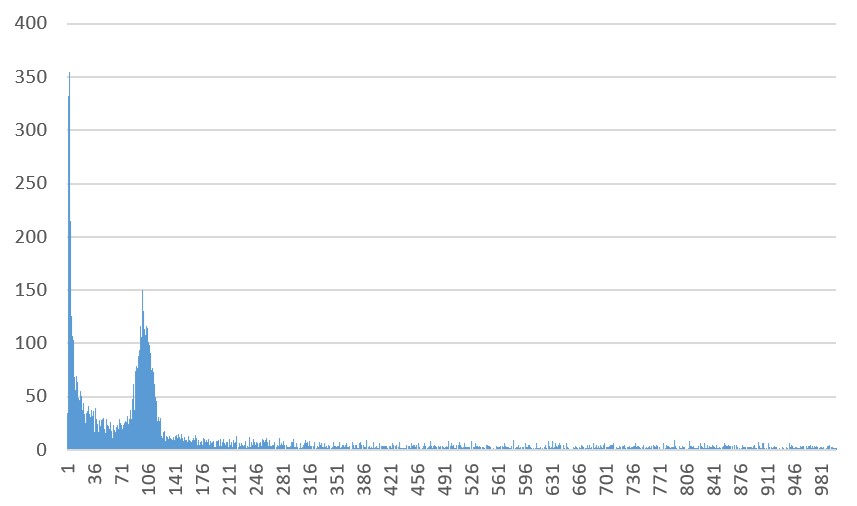
\includegraphics[width=0.7\textwidth]{figures/images/numberGenerator/mixed.png}\label{fig:mixedDistExample}
\end{figure}

The used distributions were \textasciitilde$U(1,49999)$, \textasciitilde$B(10000.0.1)$, \textasciitilde$Geo(0.001)$, powerlaw dist with $\beta=-1.25$